\documentclass[serif]{beamer}\usepackage[]{graphicx}\usepackage[]{color}
%% maxwidth is the original width if it is less than linewidth
%% otherwise use linewidth (to make sure the graphics do not exceed the margin)
\makeatletter
\def\maxwidth{ %
  \ifdim\Gin@nat@width>\linewidth
    \linewidth
  \else
    \Gin@nat@width
  \fi
}
\makeatother

\definecolor{fgcolor}{rgb}{0.345, 0.345, 0.345}
\newcommand{\hlnum}[1]{\textcolor[rgb]{0.686,0.059,0.569}{#1}}%
\newcommand{\hlstr}[1]{\textcolor[rgb]{0.192,0.494,0.8}{#1}}%
\newcommand{\hlcom}[1]{\textcolor[rgb]{0.678,0.584,0.686}{\textit{#1}}}%
\newcommand{\hlopt}[1]{\textcolor[rgb]{0,0,0}{#1}}%
\newcommand{\hlstd}[1]{\textcolor[rgb]{0.345,0.345,0.345}{#1}}%
\newcommand{\hlkwa}[1]{\textcolor[rgb]{0.161,0.373,0.58}{\textbf{#1}}}%
\newcommand{\hlkwb}[1]{\textcolor[rgb]{0.69,0.353,0.396}{#1}}%
\newcommand{\hlkwc}[1]{\textcolor[rgb]{0.333,0.667,0.333}{#1}}%
\newcommand{\hlkwd}[1]{\textcolor[rgb]{0.737,0.353,0.396}{\textbf{#1}}}%

\usepackage{framed}
\makeatletter
\newenvironment{kframe}{%
 \def\at@end@of@kframe{}%
 \ifinner\ifhmode%
  \def\at@end@of@kframe{\end{minipage}}%
  \begin{minipage}{\columnwidth}%
 \fi\fi%
 \def\FrameCommand##1{\hskip\@totalleftmargin \hskip-\fboxsep
 \colorbox{shadecolor}{##1}\hskip-\fboxsep
     % There is no \\@totalrightmargin, so:
     \hskip-\linewidth \hskip-\@totalleftmargin \hskip\columnwidth}%
 \MakeFramed {\advance\hsize-\width
   \@totalleftmargin\z@ \linewidth\hsize
   \@setminipage}}%
 {\par\unskip\endMakeFramed%
 \at@end@of@kframe}
\makeatother

\definecolor{shadecolor}{rgb}{.97, .97, .97}
\definecolor{messagecolor}{rgb}{0, 0, 0}
\definecolor{warningcolor}{rgb}{1, 0, 1}
\definecolor{errorcolor}{rgb}{1, 0, 0}
\newenvironment{knitrout}{}{} % an empty environment to be redefined in TeX

\usepackage{alltt}
\usetheme{Boadilla}
\usepackage{graphicx}
\usepackage[final]{animate}
\usepackage{breqn}
\usepackage{xcolor}
\usepackage{booktabs}
\usepackage{tikz}
\usetikzlibrary{decorations.pathreplacing}
\usetikzlibrary{shapes,arrows,positioning,shadows}
\definecolor{links}{HTML}{2A1B81}
\hypersetup{colorlinks,linkcolor=links,urlcolor=links}
\usepackage{subfig}
\usepackage{pgf}
\usepackage{pgffor}

% knitr and global options


% load R libraries


\setbeamerfont{title}{series = \bfseries}
\setbeamerfont{frametitle}{series = \bfseries} 

\newcommand{\Bigtxt}[1]{\textbf{\textit{#1}}}
\IfFileExists{upquote.sty}{\usepackage{upquote}}{}
\begin{document}

\title[Comparison of WRTDS and GAMs]{Comparison of WRTDS and GAMs for evaluating long-term trends in chlorophyll}

\author[Beck, Murphy]{Marcus W. Beck\inst{1} \and Rebecca Murphy\inst{2}}

\date{October 16, 2015}

\institute[]{\inst{1} ORISE, USEPA, Gulf Ecology Division, \href{mailto:beck.marcus@epa.gov}{beck.marcus@epa.gov} \and \inst{2} UMCES at Chesapeake Bay Program, \href{mailto:rmurphy@chesapeakebay.net}{rmurphy@chesapeakebay.net}}

%%%%%%
\begin{frame}
\titlepage
\end{frame}

%%%%%%
\begin{frame}{Since the last call...}
\begin{itemize}
\item Application of GAMs and WRTDS to 30 year time series of monthly chlorophyll at LE1.2 and TF1.6 \\~\\
\item Implementation of similar methods for model fitting \\~\\
\item Model comparisons \\~\\
\item Development of simulated datasets to evaluate flow-normalization \\~\\
\item Simulation comparisons \\~\\
\item Conclusions
\end{itemize}
\end{frame}

% chlorophyll trends by year, month, flow, combined

%%%%%%
\begin{frame}{Spatial and temporal observations}
\begin{figure}
\includegraphics<1>[width=0.8\textwidth,page=1]{figs/chlyrmofl.pdf}
\includegraphics<2>[width=0.8\textwidth,page=2]{figs/chlyrmofl.pdf}
\includegraphics<3>[width=0.8\textwidth,page=3]{figs/chlyrmofl.pdf}
\caption{Vertically integrated bi-monthly chlorophyll observations in the Patuxent, grouped by annual, seasonal, and flow periods.}
\end{figure}
\end{frame}

%%%%%%
\begin{frame}{Model applications}
LE1.2: lnchla $\sim$ time + \Bigtxt{salinity} \\~\\
TF1.6: lnchla $\sim$ time + \Bigtxt{flow} \\~\\
Fits evaluated for whole time series and annual/seasonal/flow aggregations: \\~\\
\begin{itemize}
\item predicted to observed, GAM predicted to WRTDS predicted
\item Trends in flow-normalized results (average and \% change overall, by time period) \\~\\
\end{itemize}
Model comparisons of flow-normalized results with simulated datasets
\end{frame}

%%%%%%
\begin{frame}{Parameter fitting methods}
\begin{itemize}
\item GAMs: identify optimal smoothing parameter to balance fit and `wiggliness' \\~\\
\begin{itemize}
\item Iterative generalized cross-validation with penalized likelihood maximization
\end{itemize}
\end{itemize}
\begin{itemize}
\item WRTDS: identify optimal window widths for time, discharge (salinity or flow), and season \\~\\
\begin{itemize}
\item k-fold cross-validation with search algorithm (`limited memory BFGS quasi-Newton method') that chooses window widths
\end{itemize}
\end{itemize}
\end{frame}



%%%%%%
\begin{frame}{Model comparisons}
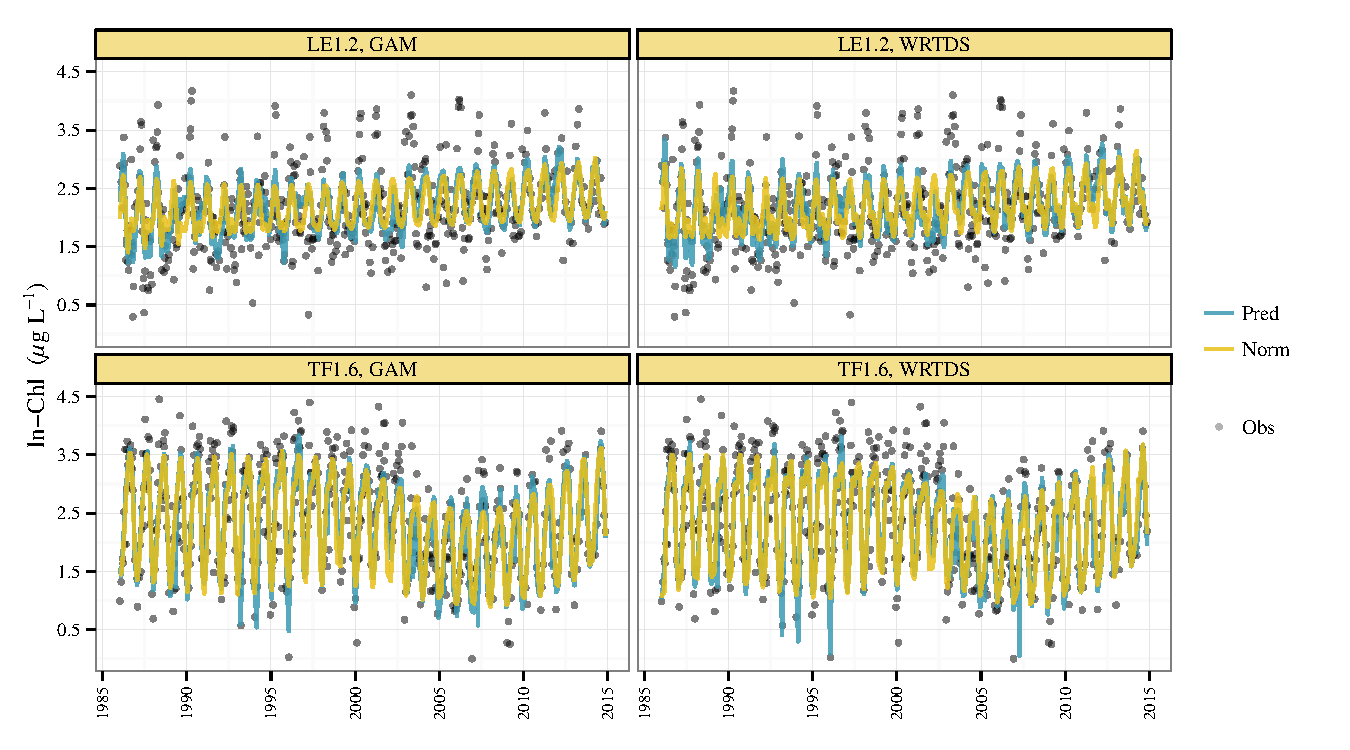
\includegraphics[width=\textwidth]{figs/predmo.pdf}
\end{frame}

%%%%%%
\begin{frame}{Model comparisons}
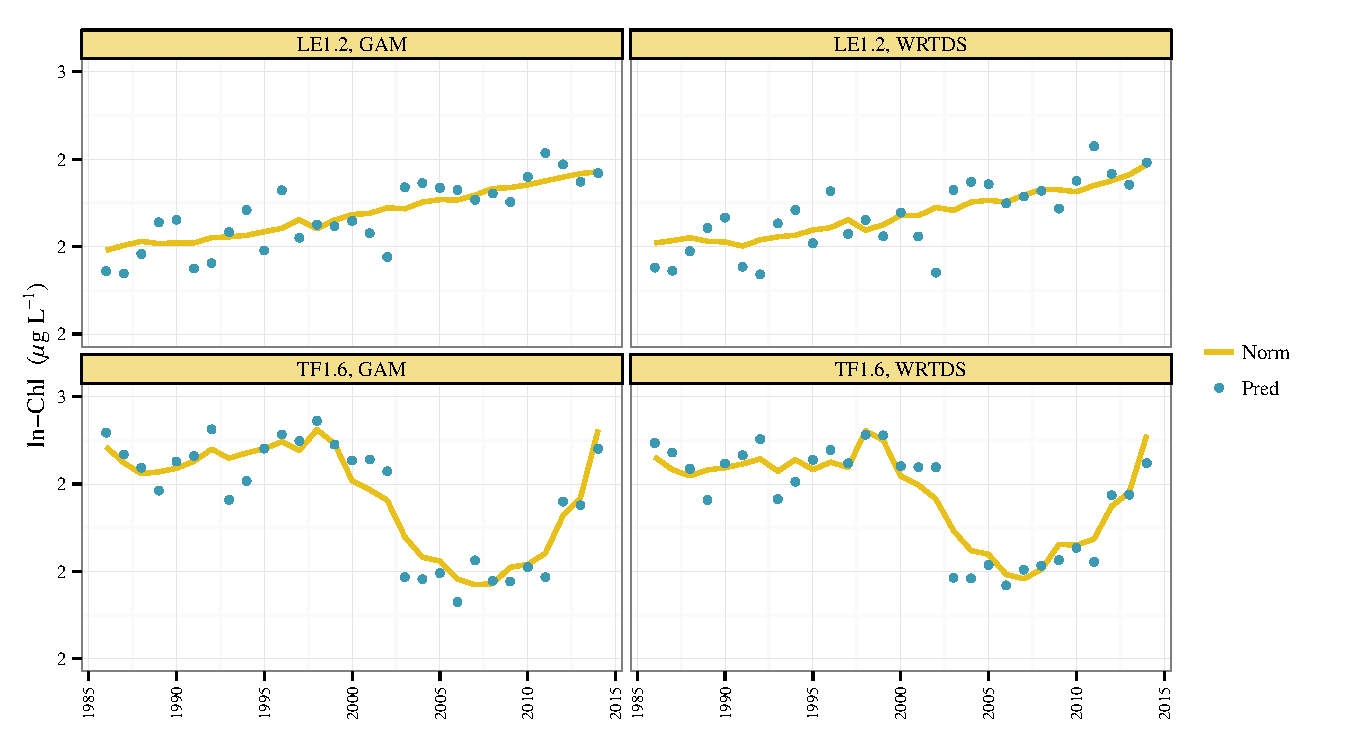
\includegraphics[width=\textwidth]{figs/predann.pdf}
\end{frame}

%%%%%%
\begin{frame}{Model comparisons}
\scriptsize
%latex.default(tab, file = "", rowlabel = "Period", caption = cap.val,     caption.loc = "top", rgroup = c("All", "Annual", "Seasonal",         "Flow"), n.rgroup = c(1, rep(4, 3)), cgroup = c("LE1.2",         "TF1.6"), n.cgroup = c(2, 2), rowname = rows, colheads = rep(c("GAM",         "WRTDS"), 2), label = "tab:perftoobs")%
\begin{table}[!tbp]
\caption{RMSE of observed to predicted ln-chlorophyll.\label{tab:perftoobs}} 
\begin{center}
\begin{tabular}{lllcll}
\hline\hline
\multicolumn{1}{l}{\bfseries Period}&\multicolumn{2}{c}{\bfseries LE1.2}&\multicolumn{1}{c}{\bfseries }&\multicolumn{2}{c}{\bfseries TF1.6}\tabularnewline
\cline{2-3} \cline{5-6}
\multicolumn{1}{l}{}&\multicolumn{1}{c}{GAM}&\multicolumn{1}{c}{WRTDS}&\multicolumn{1}{c}{}&\multicolumn{1}{c}{GAM}&\multicolumn{1}{c}{WRTDS}\tabularnewline
\hline
{\bfseries All}&&&&&\tabularnewline
~~&0.54&0.51&&0.54&0.52\tabularnewline
\hline
{\bfseries Annual}&&&&&\tabularnewline
~~1986-1993&0.54&0.50&&0.53&0.49\tabularnewline
~~1994-2000&0.52&0.50&&0.58&0.58\tabularnewline
~~2001-2007&0.63&0.60&&0.54&0.53\tabularnewline
~~2008-2014&0.39&0.36&&0.49&0.44\tabularnewline
\hline
{\bfseries Seasonal}&&&&&\tabularnewline
~~JFM&0.61&0.58&&0.53&0.49\tabularnewline
~~AMJ&0.69&0.64&&0.60&0.58\tabularnewline
~~JAS&0.38&0.35&&0.48&0.46\tabularnewline
~~OND&0.41&0.38&&0.55&0.54\tabularnewline
\hline
{\bfseries Flow}&&&&&\tabularnewline
~~1 (Low)&0.40&0.36&&0.48&0.46\tabularnewline
~~2&0.47&0.42&&0.56&0.54\tabularnewline
~~3&0.61&0.57&&0.56&0.52\tabularnewline
~~4 (High)&0.64&0.63&&0.56&0.54\tabularnewline
\hline
\end{tabular}\end{center}

\end{table}

\end{frame}

%%%%%%
\begin{frame}{Model comparisons}
\scriptsize
%latex.default(tab, file = "", rowlabel = "Period", caption = cap.val,     caption.loc = "top", rgroup = c("All", "Annual", "Seasonal",         "Flow"), n.rgroup = c(1, rep(4, 3)), cgroup = c("LE1.2",         "TF1.6"), n.cgroup = c(2, 2), rowname = rows, colheads = rep(c("Ave. diff.",         "RMSE"), 2), label = "tab:perfbtw")%
\begin{table}[!tbp]
\caption{Comparison of predicted results between models.\label{tab:perfbtw}} 
\begin{center}
\begin{tabular}{lllcll}
\hline\hline
\multicolumn{1}{l}{\bfseries Period}&\multicolumn{2}{c}{\bfseries LE1.2}&\multicolumn{1}{c}{\bfseries }&\multicolumn{2}{c}{\bfseries TF1.6}\tabularnewline
\cline{2-3} \cline{5-6}
\multicolumn{1}{l}{}&\multicolumn{1}{c}{Ave. diff.}&\multicolumn{1}{c}{RMSE}&\multicolumn{1}{c}{}&\multicolumn{1}{c}{Ave. diff.}&\multicolumn{1}{c}{RMSE}\tabularnewline
\hline
{\bfseries All}&&&&&\tabularnewline
~~&-0.11&0.15&& 0.01&0.17\tabularnewline
\hline
{\bfseries Annual}&&&&&\tabularnewline
~~1986-1993& 0.18&0.16&&-0.78&0.17\tabularnewline
~~1994-2000& 0.53&0.15&&-1.09&0.19\tabularnewline
~~2001-2007&-0.95&0.14&& 0.48&0.14\tabularnewline
~~2008-2014&-0.18&0.14&& 3.12&0.18\tabularnewline
\hline
{\bfseries Seasonal}&&&&&\tabularnewline
~~JFM& 2.91&0.14&&-5.02&0.22\tabularnewline
~~AMJ&-3.42&0.17&& 0.93&0.14\tabularnewline
~~JAS& 5.03&0.14&&-0.10&0.17\tabularnewline
~~OND&-5.25&0.14&& 2.08&0.17\tabularnewline
\hline
{\bfseries Flow}&&&&&\tabularnewline
~~Flow 1 (Low)& 0.19&0.16&&-0.09&0.12\tabularnewline
~~Flow 2&-0.83&0.16&& 0.73&0.15\tabularnewline
~~Flow 3& 0.19&0.15&& 0.84&0.20\tabularnewline
~~Flow 4 (High)& 0.03&0.13&&-1.62&0.20\tabularnewline
\hline
\end{tabular}\end{center}

\end{table}

\end{frame}

%%%%%%
\begin{frame}{Model comparisons}
\begin{knitrout}
\definecolor{shadecolor}{rgb}{0.929, 0.973, 0.984}\color{fgcolor}\begin{figure}[!ht]

{\centering 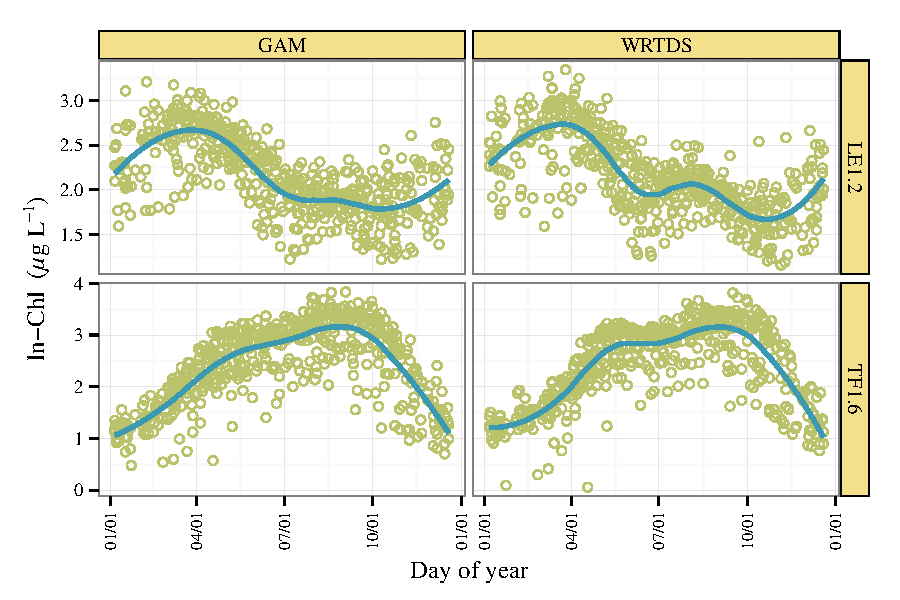
\includegraphics[width=0.9\textwidth]{figs/unnamed-chunk-6-1} 

}

\caption[Seasonal variation from model predictions]{Seasonal variation from model predictions.}\label{fig:unnamed-chunk-6}
\end{figure}


\end{knitrout}
\end{frame}



%%%%%%
\begin{frame}{Model comparisons}
\begin{figure}
\includegraphics<1>[width=\textwidth,page=2]{figs/dynaplots.pdf}
\includegraphics<2>[width=\textwidth,page=3]{figs/dynaplots.pdf}
\includegraphics<3>[width=\textwidth,page=4]{figs/dynaplots.pdf}
\includegraphics<4>[width=\textwidth,page=5]{figs/dynaplots.pdf}
\includegraphics<5>[width=\textwidth,page=6]{figs/dynaplots.pdf}
\includegraphics<6>[width=\textwidth,page=7]{figs/dynaplots.pdf}
\includegraphics<7>[width=\textwidth,page=8]{figs/dynaplots.pdf}
\includegraphics<8>[width=\textwidth,page=9]{figs/dynaplots.pdf}
\includegraphics<9>[width=\textwidth,page=10]{figs/dynaplots.pdf}
\includegraphics<10>[width=\textwidth,page=11]{figs/dynaplots.pdf}
\includegraphics<11>[width=\textwidth,page=12]{figs/dynaplots.pdf}
\includegraphics<12->[width=\textwidth,page=13]{figs/dynaplots.pdf}
\caption{Changes in the relationship between chlorophyll and flow across the time series with separate plots by month, model, and station.  The scales of salinity and flow are reversed for trend comparison with units in proportion of the total range for each month.}
\end{figure}
\end{frame}

%%%%%%
\begin{frame}{Development of simulated datasets}
\Bigtxt{Objective}: Evaluate ability of each model to reproduce flow-normalized trends\\~\\
\Bigtxt{Problem}: The true flow-normalized trends are not known and can only be empirically estimated \\~\\
We simulated monthly datasets following techniques in Beck et al. 2015 and Hirsch et al. 2015 \\~\\
\begin{itemize}
\item Daily time series: Bowie gage discharge, Jug Bay fluorescence
\item Overall: $Chl_{obs} = Chl_{flo} + Chl_{bio}$
\item Three monthly datasets with different flow components: none, constant, increasing
\end{itemize}
\end{frame}

%%%%%%
\begin{frame}{Development of simulated datasets}
Simulated data behaved as expected: three datasets with different flow contributions \\~\\
\begin{knitrout}
\definecolor{shadecolor}{rgb}{0.929, 0.973, 0.984}\color{fgcolor}\begin{figure}[!ht]

{\centering 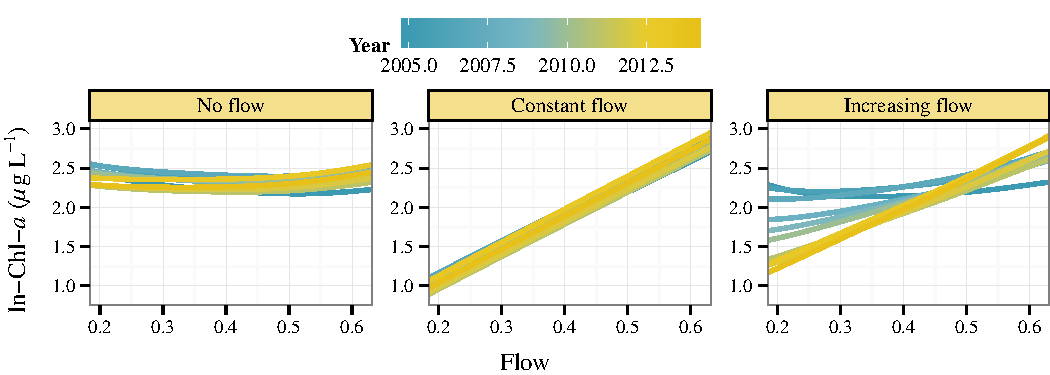
\includegraphics[width=\maxwidth]{figs/unnamed-chunk-8-1} 

}

\caption[WRTDS predictions from August for three simulated datasets with different flow contributions]{WRTDS predictions from August for three simulated datasets with different flow contributions.}\label{fig:unnamed-chunk-8}
\end{figure}


\end{knitrout}
\end{frame}

%%%%%%
\begin{frame}{Simulation comparisons}
\Bigtxt{Objective}: How well do flow-normalized predictions reproduce $Chl_{flo}$ \\~\\
Simulated time series: $Chl_{obs}$ = $Chl_{flo}$ + $Chl_{bio}$
\scriptsize
%latex.default(tab, file = "", rowlabel = "Simulations", caption = cap.val,     caption.loc = "top", rgroup = c("No flow", "Constant flow",         "Increasing flow"), n.rgroup = rep(2, 3), rowname = rows,     colheads = c("$Chl_{obs} \\sim \\widehat{Chl}_{obs}$", "$Chl_{bio} \\sim \\widehat{Chl}_{bio}$"),     label = "tab:simperf")%
\begin{table}[!tbp]
\caption{Performance summaries (RMSE) of model predictions for the three simulated time series.\label{tab:simperf}} 
\begin{center}
\begin{tabular}{lll}
\hline\hline
\multicolumn{1}{l}{Simulations}&\multicolumn{1}{c}{$Chl_{obs} \sim \widehat{Chl}_{obs}$}&\multicolumn{1}{c}{$Chl_{bio} \sim \widehat{Chl}_{bio}$}\tabularnewline
\hline
{\bfseries No flow}&&\tabularnewline
~~GAM&0.51&0.53\tabularnewline
~~WRTDS&0.50&0.52\tabularnewline
\hline
{\bfseries Constant flow}&&\tabularnewline
~~GAM&0.51&0.58\tabularnewline
~~WRTDS&0.53&0.57\tabularnewline
\hline
{\bfseries Increasing flow}&&\tabularnewline
~~GAM&0.51&0.54\tabularnewline
~~WRTDS&0.50&0.52\tabularnewline
\hline
\end{tabular}\end{center}

\end{table}

\end{frame}

%%%%%%
\begin{frame}{Conclusions}
\begin{itemize}
\item WRTDS prediction errors always less than GAMs \\~\\
\item Seasonal patterns were slightly different between models \\~\\
\item GAM estimates were more `stable' during periods with little data \\~\\
\item No clear differences in flow-normalization abilities \\~\\
\item Interesting trends in Patuxent \\~\\
\begin{itemize}
\item Chlorophyll increasing lower estuary (LE1.2), mainstem influences
\item Multi-year signal of Isabel at TF1.6, flushing and low chlorophyll
\item Distinct changing relationships of chlorophyll with flow by station
\end{itemize}
\end{itemize}
\end{frame}

%%%%%%
\begin{frame}{Conclusions}
Journal venue?  Modelling vs ecosystem dynamics? Two papers?
\end{frame}

%%%%%%
\begin{frame}{Extra}
For comparing each model's \Bigtxt{predictions to observed}, at both sites:\\~\\
\begin{center}
$RMSE_{fit} = \sqrt {\frac{{\sum\limits_{{i = 1}}^n {{{\left( {{Chl_i} - {\widehat{Chl}_i}} \right)}^2}} }}{n}}$
\end{center}
For comparing \Bigtxt{predictions between models}, at both sites: \\~\\
\begin{center} 
$RMSE_{btw} = \sqrt {\frac{{\sum\limits_{{i = 1}}^n {{{\left( {{\widehat{Chl}_{WRTDS,\,i}} - {{\widehat{Chl}}_{GAM,\,i}}} \right)}^2}} }}{n}}$
\end{center}
\begin{center}
$\textrm{Average difference} = \left(\frac{\sum\limits_{i = 1}^n \widehat{Chl}_{WRTDS,\,i} - \sum\limits_{i = 1}^n \widehat{Chl}_{GAM,\,i}}{\sum\limits_{i = 1}^n \widehat{Chl}_{GAM,\,i}}\right) * 100$
\end{center}
\end{frame}

%%%%%%
\begin{frame}{Extra}
Simulated datasets:\\~\\
\begin{itemize}
\item Daily time series: Bowie gage discharge, Jug Bay fluorescence
\item Overall: $Chl_{obs} = Chl_{flo} + Chl_{bio}$
\item From discharge: $Chl_{flo} = I\left(\widehat{Q}_{seas} + \sigma\cdot\varepsilon_{Q,\,sim}\right)$
\item From fluorescence: $Chl_{bio} = \widehat{Chl}_{seas} + \sigma\cdot\varepsilon_{Chl,\,sim}$
\item Indicator $I$ changes to simulate changing flow component
\end{itemize}
\end{frame}

%%%%%%
\begin{frame}[fragile]{Extra}
\begin{knitrout}
\definecolor{shadecolor}{rgb}{0.929, 0.973, 0.984}\color{fgcolor}

{\centering 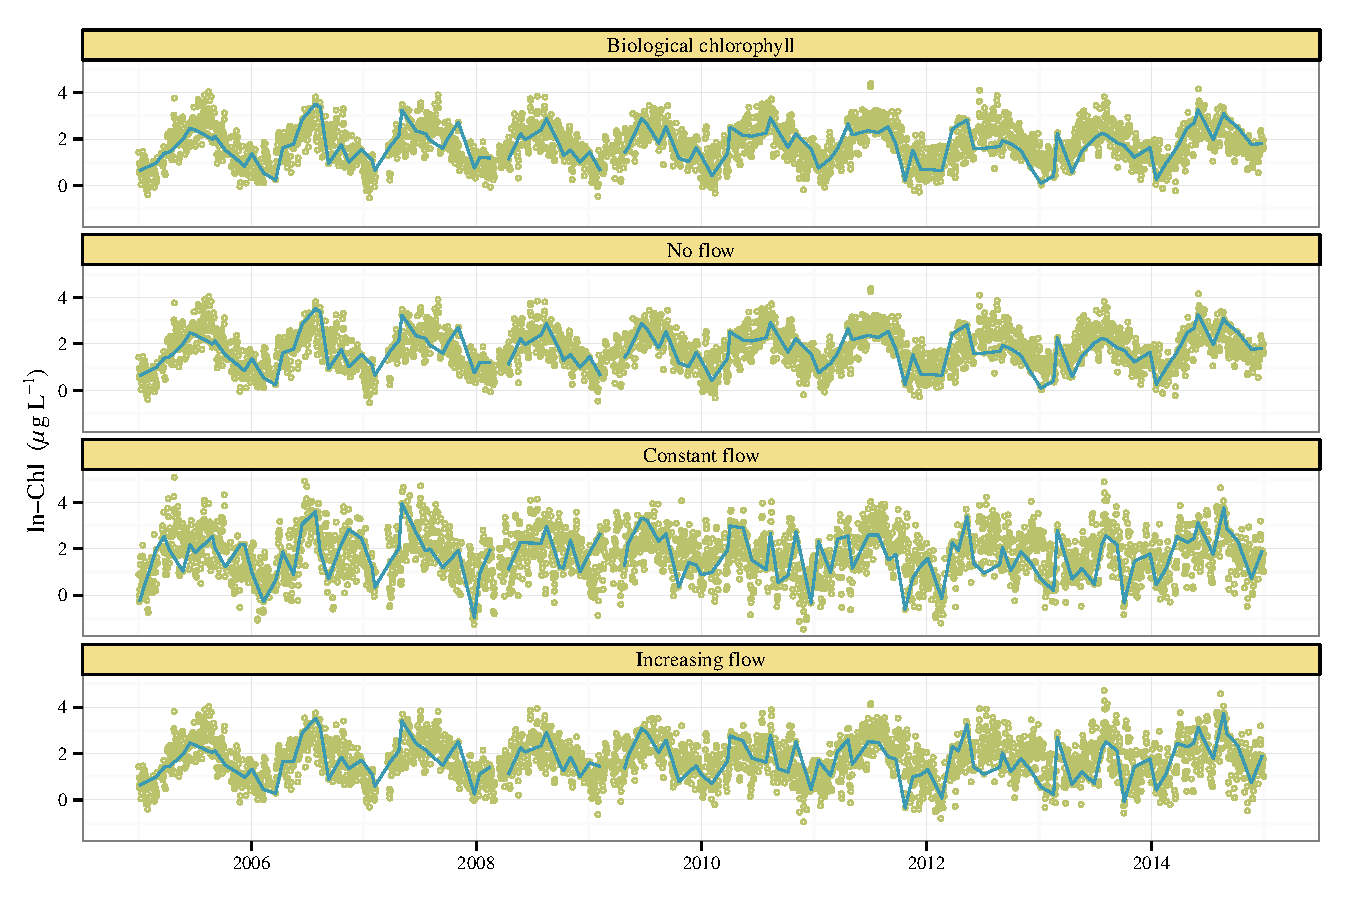
\includegraphics[width=\maxwidth]{figs/unnamed-chunk-10-1} 

}



\end{knitrout}
\end{frame}

\end{document}
